%==========================================================
% Beamer mini-deck (house-style friendly)
% Topic: Mechanistic interpretability -> Patching -> Graph dataset -> Classical/Quantum Kernels
% Improvements requested:
% (1) Motivation reframed as *the mechanistic interpretability problem* (not project selection).
% (2) Clear patching slide + formal theory under "Theoretical Formulation", with TikZ conceptual drawings.
% (3) After Algorithm 3: new section with a step-by-step execution plan (slides per task: what/how/expect).
%==========================================================

\documentclass[aspectratio=169,xcolor={dvipsnames}]{beamer}
\usetheme{Madrid}
\IfFileExists{beamercolorthemeDusk.sty}{%
\usecolortheme{Dusk}
}{%
\usecolortheme{default}
}

\renewcommand{\accent}[1]{\textbf{#1}}
\newcommand{\smalltitle}[1]{\textbf{#1}}

\usepackage{amsmath,amssymb,amsthm}
\usepackage{mathtools}
\usepackage{bm}
\IfFileExists{algorithm2e.sty}{%
\usepackage[ruled,vlined]{algorithm2e}
}{%
\newenvironment{algorithm}[1][]{\begin{center}\begin{minipage}{0.95\linewidth}\small}{\end{minipage}\end{center}}
\newcommand{\DontPrintSemicolon}{}
\newcommand{\SetAlgoLined}{}
\newcommand{\SetKwInOut}[2]{\expandafter\newcommand\csname #1\endcsname[1]{\par\textbf{#2:} ##1\par}}
\newcommand{\BlankLine}{\par\smallskip}
\newcommand{\For}[2]{\par\textbf{for} #1 #2\par}
\newcommand{\uIf}[2]{\par\textbf{if} #1 #2\par}
\newcommand{\ElseIf}[2]{\par\textbf{else if} #1 #2\par}
\newcommand{\tcp}[1]{\emph{#1}\par}
\renewcommand{\caption}[1]{\par\smallskip\textbf{#1}\par}
}
\usepackage{tikz}
\usetikzlibrary{arrows.meta,calc,positioning,fit,backgrounds,shapes.geometric}
\usepackage{graphicx}
\usepackage{multicol}

\usepackage{listings}
% \usepackage{xcolor}
% \usepackage[T1]{fontenc}
% \usepackage{lmodern}
\tikzset{>=Latex}

% Code styling
\definecolor{codegreen}{rgb}{0,0.6,0}
\definecolor{codegray}{rgb}{0.5,0.5,0.5}
\definecolor{codepurple}{rgb}{0.58,0,0.82}
\definecolor{backcolour}{rgb}{0.95,0.95,0.92}

\lstdefinestyle{pythonstyle}{
  language=Python,
  backgroundcolor=\color{backcolour},
  basicstyle=\ttfamily\small,
  commentstyle=\color{codegreen},
  keywordstyle=\color{blue},
  numberstyle=\tiny\color{codegray},
  stringstyle=\color{codepurple},
  numbers=left,
  numbersep=5pt,
  showstringspaces=false,
  breaklines=true,
  tabsize=4,
  columns=fullflexible,
  keepspaces=true,
}

\lstset{style=pythonstyle}



\DeclareMathOperator{\Tr}{Tr}
\DeclareMathOperator{\Exp}{\mathbb{E}}

\newcommand{\R}{\mathbb{R}}
\newcommand{\N}{\mathbb{N}}

\title[Patching Kernels]{Patching-based Interpretability Graphs \\ and Kernel Methods}
\subtitle{Mechanistic Interpretability $\rightarrow$ Graph Datasets $\rightarrow$ Similarity Geometry}
\author{MI Working Group}
\institute{Uvigo}
\date{}

% ---------------------------------------------------------
% TikZ styles (conceptual drawings)
% ---------------------------------------------------------
\tikzset{
  box/.style={rounded corners, draw, thick, fill=white, inner sep=6pt, align=center},
  sbox/.style={rounded corners, draw, thick, fill=white, inner sep=4pt, align=center},
  arrow/.style={-Latex, thick},
  dashedarrow/.style={-Latex, thick, dashed},
  highlight/.style={draw=RoyalBlue, very thick, rounded corners},
  faint/.style={draw=black!30, thick, rounded corners},
}

\begin{document}

\frame{\titlepage}

\begin{frame}[shrink=16]{Roadmap}
\tableofcontents
\end{frame}

%==========================================================
\section{Problem Setting: Mechanistic Interpretability}
%==========================================================



\begin{frame}[shrink=20]{Motivation: Mechanistic Interpretability as a \emph{causal structure discovery}}
    \small
    \begin{columns}[T,onlytextwidth]
    %---------------------- LEFT COLUMN ----------------------%
    \begin{column}{0.54\textwidth}
    \begin{block}{Problem statement (why patching exists)}
    Transformer models implement complex computations distributed across
    \accent{layers, tokens, heads, and MLPs}. Mechanistic interpretability asks:
    \begin{itemize}\setlength\itemsep{3pt}
    \item \accent{Which internal components causally influence} a target behavior (e.g., next-token logit)?
    \item \accent{How do components compose into circuits} that implement the computation?
    \item \accent{How stable are these circuits} across prompts, corruptions, and noise?
    \end{itemize}
    \end{block}

    \begin{block}{Key obstacle}
    Purely observational probes (activations, correlations) confound
    \emph{co-activation} with \emph{causal influence}. We need \accent{interventions}
    to map \emph{cause $\rightarrow$ effect} inside the network.
    \end{block}
    \end{column}

    %---------------------- RIGHT COLUMN ---------------------%
    \begin{column}{0.44\textwidth}
    \begin{block}{Core idea of this project}
    Use patching to produce a \accent{large interventional dataset}, summarize it
    as a \accent{graph dataset}, then use kernels (classical / quantum) to learn an
    \accent{effective similarity geometry} over circuits.
    \end{block}

    \vspace{1mm}
    \begin{center}
    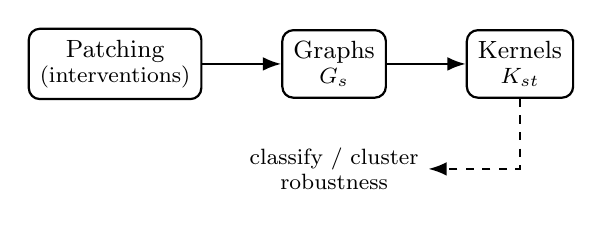
\begin{tikzpicture}[node distance=7mm]
    \node[rounded corners, draw, thick, align=center, inner sep=4pt] (patch)
    {\small Patching\\[-1mm]\footnotesize (interventions)};
    \node[rounded corners, draw, thick, right=10mm of patch, align=center, inner sep=4pt] (graph)
    {\small Graphs\\[-1mm]\footnotesize $G_s$};
    \node[rounded corners, draw, thick, right=10mm of graph, align=center, inner sep=4pt] (kern)
    {\small Kernels\\[-1mm]\footnotesize $K_{st}$};

    \draw[-Latex, thick] (patch) -- (graph);
    \draw[-Latex, thick] (graph) -- (kern);

    \node[below=5mm of graph, align=center] (tasks)
    {\footnotesize classify / cluster\\[-1mm]\footnotesize robustness};
    \draw[-Latex, thick, dashed] (kern) |- (tasks);
    \end{tikzpicture}
    \end{center}
    \end{column}
    \end{columns}
\end{frame}



\begin{frame}[shrink=20]{Conceptual pipeline (from interventions to a learnable dataset)}
\small
\centering

\newcommand{\pipestep}{9mm} % <-- reduce/increase to fit (e.g. 9mm, 10mm, 12mm, 14mm)

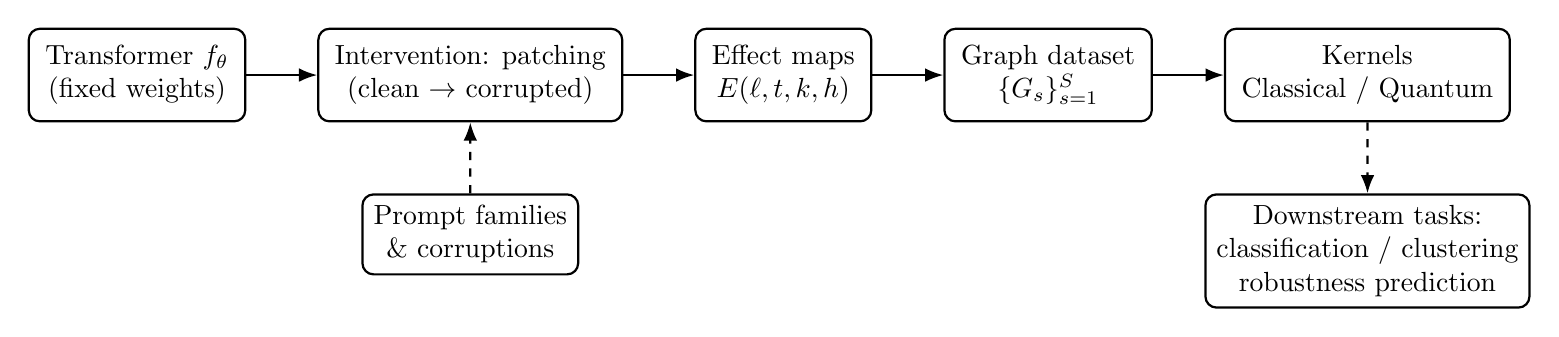
\begin{tikzpicture}[scale=0.6,node distance=9mm]
\node[box] (model) {Transformer $f_\theta$\\(fixed weights)};
\node[box, right=\pipestep of model] (patch) {Intervention: patching\\(clean $\rightarrow$ corrupted)};
\node[box, right=\pipestep of patch] (effects) {Effect maps\\$E(\ell,t,k,h)$};
\node[box, right=\pipestep of effects] (graphs) {Graph dataset\\$\{G_s\}_{s=1}^S$};
\node[box, right=\pipestep of graphs] (kernels) {Kernels\\Classical / Quantum};

\draw[arrow] (model) -- (patch);
\draw[arrow] (patch) -- (effects);
\draw[arrow] (effects) -- (graphs);
\draw[arrow] (graphs) -- (kernels);

\node[sbox, below=9mm of patch] (data) {Prompt families\\\& corruptions};
\draw[dashedarrow] (data) -- (patch);

\node[sbox, below=9mm of kernels] (tasks) {Downstream tasks:\\classification / clustering\\robustness prediction};
\draw[dashedarrow] (kernels) -- (tasks);
\end{tikzpicture}



\vspace{2mm}
\begin{block}{What becomes the dataset?}
Each slice $s$ (task family, corruption type, prompt family) yields one graph $G_s$.
Learning happens \emph{across graphs}, not just within a single prompt.
\end{block}
\end{frame}

%==========================================================
\section{Patching: From Interventions to Effect Maps}
%==========================================================



\begin{frame}[shrink=20]{Patching: controlled interventions inside the forward pass}
\small
\begin{columns}[T,onlytextwidth]
%---------------------- LEFT COLUMN ----------------------%
\begin{column}{0.54\textwidth}
\begin{block}{Clean vs corrupted runs}
For each example $i$, we build a pair:
\[
(x_i^{\mathrm{cln}},\; x_i^{\mathrm{crp}}),
\]
where $x_i^{\mathrm{crp}}$ is designed to break the target behavior while preserving structure.
\end{block}

\begin{block}{Effect size (scalar observable)}
Let $O(\cdot)$ be a scalar observable (logit, log-prob, loss). Define the patch effect:
\[
E_u(x^{\mathrm{cln}},x^{\mathrm{crp}})
\;=\;
O\!\left(\tilde f_\theta(x^{\mathrm{crp}};u)\right)-O\!\left(f_\theta(x^{\mathrm{crp}})\right).
\]
Large $E_u$ means that intervening at $u$ causally restores the target behavior.
\end{block}


\end{column}

%---------------------- RIGHT COLUMN ---------------------%
\begin{column}{0.44\textwidth}

\begin{block}{Activation patching (local intervention)}
Choose an internal node $u$ (layer/token/component/head). Run the corrupted forward pass, but
\accent{replace} the activation at $u$ with the corresponding clean activation.
\end{block}


\begin{block}{Conceptual diagram}
\centering
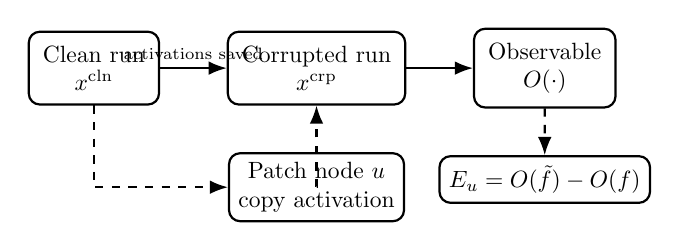
\begin{tikzpicture}[node distance=10mm, scale=0.85, transform shape]
\node[box] (clean) {Clean run\\$x^{\mathrm{cln}}$};
\node[box, right=10mm of clean] (corr) {Corrupted run\\$x^{\mathrm{crp}}$};
\node[box, right=10mm of corr] (obs) {Observable\\$O(\cdot)$};

\draw[arrow] (clean) -- node[above]{\scriptsize activations saved} (corr);
\draw[arrow] (corr) -- (obs);

\node[sbox, below=7mm of corr] (nodeu) {Patch node $u$\\copy activation};
\draw[dashedarrow] (clean) |- (nodeu);
\draw[dashedarrow] (nodeu) -| (corr);

\node[sbox, below=7mm of obs] (delta) {$E_u = O(\tilde f)-O(f)$};
\draw[dashedarrow] (obs) -- (delta);
\end{tikzpicture}
\end{block}
\end{column}
\end{columns}
\end{frame}




%==========================================================
\section{Theoretical Formulation}
%==========================================================




\begin{frame}[shrink=28]{Formal setup: model, observable, and component activations}
\small
\begin{columns}[T,onlytextwidth]
%---------------------- LEFT COLUMN ----------------------%
\begin{column}{0.54\textwidth}
\begin{block}{Model and observable}
Let $f_\theta$ be a transformer. For a prompt $x=(x_1,\dots,x_T)$, denote logits by
$\bm{\ell}(x)\in\R^{|V|}$. Choose an observable:
\[
O(x)=\ell_{y^\star}(x)
\quad\text{or}\quad
O(x)=-\log p_\theta(y^\star\mid x),
\]
where $y^\star$ is the target token.
\end{block}

\begin{block}{Component types and indices}
Let $\ell\in\{0,\dots,L-1\}$ (layer), $t\in\{1,\dots,T\}$ (token index),
\[
\mathcal{K} \coloneqq \{\textsf{res},\ \textsf{att},\ \textsf{mlp}\},
\qquad
h\in\{1,\dots,H\}\ \text{(heads, only for }\textsf{att}\text{)}.
\]
Example activations:
\[
a_{\ell,t}^{\textsf{res}}(x)\in\R^d,\quad
a_{\ell,t,h}^{\textsf{att}}(x)\in\R^d,\quad
a_{\ell,t}^{\textsf{mlp}}(x)\in\R^d.
\]
\end{block}
\end{column}

%---------------------- RIGHT COLUMN ---------------------%
\begin{column}{0.42\textwidth}
\begin{block}{Conceptual view (what is indexed by $(\ell,t,k,h)$?)}
\centering
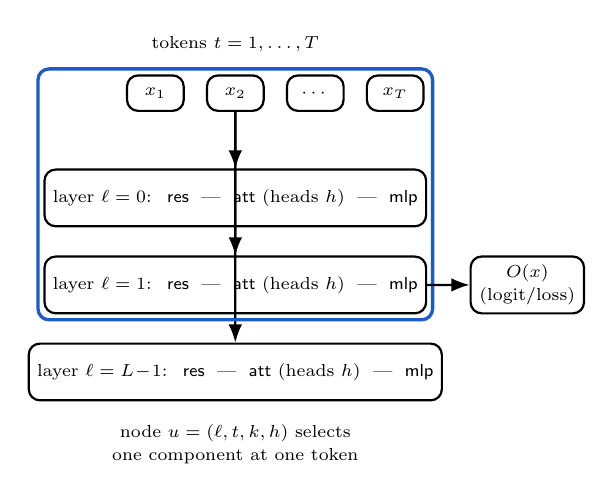
\begin{tikzpicture}[scale=0.9, transform shape, node distance=6mm]
% tokens row
\node[draw, rounded corners, thick, minimum width=8mm, minimum height=5mm] (t1) {\scriptsize $x_1$};
\node[draw, rounded corners, thick, right=3mm of t1, minimum width=8mm, minimum height=5mm] (t2) {\scriptsize $x_2$};
\node[draw, rounded corners, thick, right=3mm of t2, minimum width=8mm, minimum height=5mm] (t3) {\scriptsize $\cdots$};
\node[draw, rounded corners, thick, right=3mm of t3, minimum width=8mm, minimum height=5mm] (tT) {\scriptsize $x_T$};
\node[above=2mm of t2, align=center] {\scriptsize tokens $t=1,\dots,T$};

% layer stack (schematic)
\node[draw, rounded corners, thick, fill=white, below=8mm of t2, minimum width=42mm, minimum height=8mm, align=center] (l0)
{\scriptsize layer $\ell=0$: \ \textsf{res} \;|\; \textsf{att} (heads $h$) \;|\; \textsf{mlp}};
\node[draw, rounded corners, thick, fill=white, below=4mm of l0, minimum width=42mm, minimum height=8mm, align=center] (l1)
{\scriptsize layer $\ell=1$: \ \textsf{res} \;|\; \textsf{att} (heads $h$) \;|\; \textsf{mlp}};
\node[draw, rounded corners, thick, fill=white, below=4mm of l1, minimum width=42mm, minimum height=8mm, align=center] (l2)
{\scriptsize layer $\ell=L\!-\!1$: \ \textsf{res} \;|\; \textsf{att} (heads $h$) \;|\; \textsf{mlp}};

% arrows from token to layers (index t selects a column through depth)
\draw[-Latex, thick] (t2) -- (l0.north);
\draw[-Latex, thick] (t2) -- (l1.north);
\draw[-Latex, thick] (t2) -- (l2.north);

% highlight a "node" u = (l,t,k,h): use explicit RGB instead of RoyalBlue
\node[draw={rgb,255:red,30;green,90;blue,200}, very thick, rounded corners, inner sep=2pt,
      fit=(t2) (l1)] (u) {};

\node[below=2mm of l2, align=center]
{\scriptsize node $u=(\ell,t,k,h)$ selects\\[-1mm]\scriptsize one component at one token};

% observable
\node[draw, rounded corners, thick, right=6mm of l1, minimum width=16mm, minimum height=8mm, align=center] (obs)
{\scriptsize $O(x)$\\[-1mm]\scriptsize (logit/loss)};
\draw[-Latex, thick] (l1.east) -- (obs.west);

\end{tikzpicture}
\end{block}
\end{column}
\end{columns}
\end{frame}




\begin{frame}[shrink=34]{Nodes \& graphs: mathematical definition (what the dataset actually is)}
\small
\begin{columns}[T,onlytextwidth]
%---------------------- LEFT COLUMN ----------------------%
\begin{column}{0.58\textwidth}
\begin{block}{Node set (mechanistic granularity)}
Fix $(L,T,H)$. Define the node set as a disjoint union:
\[
\mathcal{V}
=
\mathcal{V}_{\textsf{res}}
\;\dot\cup\;
\mathcal{V}_{\textsf{mlp}}
\;\dot\cup\;
\mathcal{V}_{\textsf{att}},
\]
where
\[
\mathcal{V}_{\textsf{res}}=\{(\ell,t,\textsf{res}) : 0\le \ell<L,\ 1\le t\le T\},
\quad
\mathcal{V}_{\textsf{mlp}}=\{(\ell,t,\textsf{mlp}) : 0\le \ell<L,\ 1\le t\le T\},
\]
\[
\mathcal{V}_{\textsf{att}}=\{(\ell,t,h,\textsf{att}) : 0\le \ell<L,\ 1\le t\le T,\ 1\le h\le H\}.
\]
A generic node is $u\in\mathcal{V}$.
\end{block}

\begin{block}{Graph per slice}
For each slice $s$ (task family / corruption type / prompt family), build a directed weighted graph:
\[
G_s = (\mathcal{V},\mathcal{E}_s,w_s).
\]
Weights $w_s(u\!\to\!v)$ are computed from patch-effect profiles across examples in slice $s$.
\end{block}
\end{column}

%---------------------- RIGHT COLUMN ---------------------%
\begin{column}{0.40\textwidth}
\begin{block}{Conceptual view (fixed nodes, varying edges by slice)}
\centering
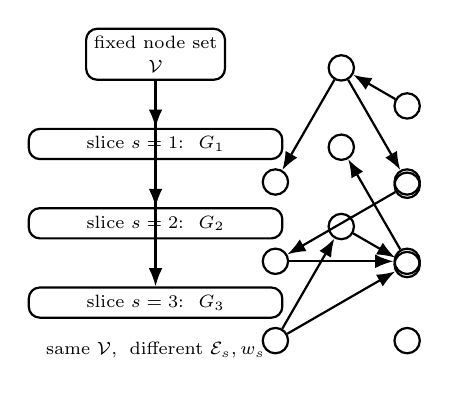
\begin{tikzpicture}[scale=0.92, transform shape]
% --- knobs ---
\def\nrad{1.05cm}   % radius of the node-ring
\def\ssep{6.5mm}    % vertical separation between slice-graphs

% --- a common node set (ring) ---
\node[draw, rounded corners, thick, align=center, inner sep=3pt] (V)
{\scriptsize fixed node set\\[-1mm]\scriptsize $\mathcal{V}$};

% Slice graphs as "edge patterns" over the same nodes
\node[draw, rounded corners, thick, below=\ssep of V, inner sep=3pt, minimum width=35mm] (G1)
{\scriptsize slice $s=1$:\; $G_1$};
\node[draw, rounded corners, thick, below=\ssep of G1, inner sep=3pt, minimum width=35mm] (G2)
{\scriptsize slice $s=2$:\; $G_2$};
\node[draw, rounded corners, thick, below=\ssep of G2, inner sep=3pt, minimum width=35mm] (G3)
{\scriptsize slice $s=3$:\; $G_3$};

\draw[-Latex, thick] (V) -- (G1);
\draw[-Latex, thick] (V) -- (G2);
\draw[-Latex, thick] (V) -- (G3);

% Small schematic "graph" icons on the right of each slice box
\foreach \name/\y in {gA/0, gB/1, gC/2} {
  % anchor point to the right of each slice label
}

% --- icon for G1 ---
\begin{scope}[shift={(G1.east)}, xshift=8mm]
  \foreach \i/\ang in {1/90,2/210,3/330,4/30}{
    \node[circle, draw, thick, minimum size=3.5mm] (a\i) at (\ang:\nrad) {};
  }
  \draw[-Latex, thick] (a1) -- (a2);
  \draw[-Latex, thick] (a1) -- (a3);
  \draw[-Latex, thick] (a4) -- (a1);
\end{scope}

% --- icon for G2 ---
\begin{scope}[shift={(G2.east)}, xshift=8mm]
  \foreach \i/\ang in {1/90,2/210,3/330,4/30}{
    \node[circle, draw, thick, minimum size=3.5mm] (b\i) at (\ang:\nrad) {};
  }
  \draw[-Latex, thick] (b2) -- (b3);
  \draw[-Latex, thick] (b3) -- (b1);
  \draw[-Latex, thick] (b4) -- (b2);
\end{scope}

% --- icon for G3 ---
\begin{scope}[shift={(G3.east)}, xshift=8mm]
  \foreach \i/\ang in {1/90,2/210,3/330,4/30}{
    \node[circle, draw, thick, minimum size=3.5mm] (c\i) at (\ang:\nrad) {};
  }
  \draw[-Latex, thick] (c1) -- (c4);
  \draw[-Latex, thick] (c2) -- (c1);
  \draw[-Latex, thick] (c2) -- (c4);
\end{scope}

% Caption at bottom
\node[align=center, below=2mm of G3] {\scriptsize same $\mathcal{V}$,\; different $\mathcal{E}_s,w_s$};

\end{tikzpicture}
\end{block}
\end{column}
\end{columns}
\end{frame}



\begin{frame}[shrink=38]{From patch effects to graphs: two principled constructions}
\small
\begin{columns}[T,onlytextwidth]
%---------------------- LEFT COLUMN ----------------------%
\begin{column}{0.58\textwidth}
\begin{block}{(A) Influence-to-output graph (direct causal score)}
Define node score as the expected causal restoration:
\[
\mathrm{score}_s(u) \;=\; \Exp_{i\in\mathcal{I}_s}\!\left[E_u^{(i)}\right],
\]
and define directed edges by conditional/paired interventions (optional extension):
\[
w_s(u\to v)\approx \Exp\!\left[ E_{u\ \text{then}\ v} - E_{u} \right],
\]
capturing how $v$ mediates the effect of $u$.
\end{block}

\begin{block}{(B) Co-influence graph (robust, cheap, dataset-friendly)}
Given patch-effect vectors $\{E_u^{(i)}\}_{i\in\mathcal{I}_s}$, define
\[
w_s(u\to v)
=
\mathrm{corr}\!\left(\{E_u^{(i)}\}_{i\in\mathcal{I}_s},\ \{E_v^{(i)}\}_{i\in\mathcal{I}_s}\right),
\quad\text{often use}\quad |w_s(u\to v)|.
\]
Interpretation: nodes whose interventions co-vary across prompts behave as a coherent circuit.
\end{block}

\begin{block}{Direction constraint (recommended)}
Allow edges only from earlier to later in a partial order $\prec$ (e.g.\ by layer, then token):
\[
(u\to v)\in\mathcal{E}_s \Rightarrow u\prec v.
\]
\end{block}
\end{column}

%---------------------- RIGHT COLUMN ---------------------%
\begin{column}{0.40\textwidth}

%==================== Knobs (tweak these) ====================%
\newcommand{\panelScale}{0.88}   % overall scale for BOTH panels
\newcommand{\xA}{11mm}           % horizontal spacing in panel (A)
\newcommand{\yA}{12mm}            % vertical spacing in panel (A)
\newcommand{\xB}{14mm}           % horizontal spacing in panel (B)
\newcommand{\yB}{12mm}            % vertical spacing in panel (B)
\newcommand{\stackSep}{3mm}      % vertical separation between (A) and (B) panels
\newcommand{\nodeSize}{4.2mm}    % circle node size
%=============================================================%

\tikzset{
  n/.style={circle, draw, thick, minimum size=2*\nodeSize, inner sep=0pt},
  rbox/.style={draw, rounded corners, thick, align=center, inner sep=3pt},
  lab/.style={font=\scriptsize, align=center},
}

\begin{block}{Conceptual view (edge definitions)}
\centering

%--------------------- Panel (A) ---------------------%
\begin{tikzpicture}[scale=\panelScale, transform shape]
\node[lab] (titleA) at (0,0) {\textbf{(A)} Influence-to-output (mediation)};

\node[n] (u)  at (-\xA, -\yA) {\scriptsize $u$};
\node[n] (v)  at (0,   -\yA) {\scriptsize $v$};
\node[rbox] (O) at (\xA, -\yA) {\scriptsize $O$};

\draw[-Latex, thick] (u) -- (v);
\draw[-Latex, thick] (v) -- (O);

\node[rbox] (pair) at (0, -2.25*\yA)
{\scriptsize paired patches\\[-1mm]\scriptsize compare $E_u$ vs $E_{u\ \text{then}\ v}$};
\draw[-Latex, thick, dashed] (pair) -- (v);

\node[lab] at (0, -0.25*\yA)
{\scriptsize $w(u\!\to\!v)\approx \Exp[E_{u\ \text{then}\ v}-E_u]$};

% optional direction hint
\node[lab] at (0, -3.05*\yA) {\scriptsize (often keep only $u\prec v$)};
\end{tikzpicture}

\vspace{\stackSep}

%--------------------- Panel (B) ---------------------%
\begin{tikzpicture}[scale=\panelScale, transform shape]
\node[lab] (titleB) at (0,0) {\textbf{(B)} Co-influence (correlation of profiles)};

\node[n] (u2) at (-\xB, -\yB) {\scriptsize $u$};
\node[n] (v2) at ( \xB, -\yB) {\scriptsize $v$};

\node[rbox] (Eu) at (-\xB, -2.25*\yB) {\scriptsize $\{E_u^{(i)}\}_i$};
\node[rbox] (Ev) at ( \xB, -2.25*\yB) {\scriptsize $\{E_v^{(i)}\}_i$};
\node[rbox] (corr) at (0, -2.25*\yB) {\scriptsize $\mathrm{corr}$};

\draw[-Latex, thick] (Eu) -- (u2);
\draw[-Latex, thick] (Ev) -- (v2);
\draw[-Latex, thick] (Eu.east) -- (corr.west);
\draw[-Latex, thick] (Ev.west) -- (corr.east);

\draw[-Latex, thick] (u2) -- node[above, font=\scriptsize] {$|w|$} (v2);

\node[lab] at (0, -0.25*\yB)
{\scriptsize $w(u\!\to\!v)=\mathrm{corr}(E_u,E_v)$};
\node[lab] at (0, -3.05*\yB) {\scriptsize (then sparsify: top-$k$ edges per node)};
\end{tikzpicture}

\end{block}
\end{column}
\end{columns}
\end{frame}




\begin{frame}[shrink=20]{Edge sparsification \& comparability (make graphs scalable)}
\small
\begin{block}{Top-$k$ sparsification (critical)}
For each $u\in\mathcal{V}$, keep only top-$k$ outgoing edges by $|w_s(u\to v)|$:
\[
\mathcal{E}_s
=
\bigcup_{u\in\mathcal{V}}
\left\{(u\to v) : v \in \mathrm{TopK}_k\big(\{|w_s(u\to \cdot)|\}\big)\right\}.
\]
This fixes graph size and stabilizes downstream kernels.
\end{block}

\begin{block}{Conceptual view (same nodes, different slices)}
\centering
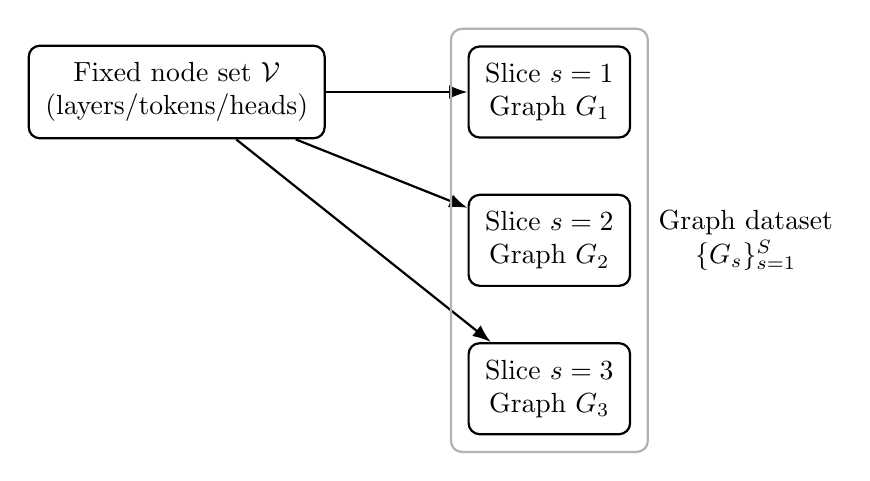
\begin{tikzpicture}[node distance=9mm]
\node[box] (nodes) {Fixed node set $\mathcal{V}$\\(layers/tokens/heads)};
\node[box, right=18mm of nodes] (slice1) {Slice $s=1$\\Graph $G_1$};
\node[box, below=7mm of slice1] (slice2) {Slice $s=2$\\Graph $G_2$};
\node[box, below=7mm of slice2] (slice3) {Slice $s=3$\\Graph $G_3$};

\draw[arrow] (nodes) -- (slice1);
\draw[arrow] (nodes) -- (slice2);
\draw[arrow] (nodes) -- (slice3);

\node[faint, fit=(slice1)(slice2)(slice3), inner sep=6pt, label={[align=center]right:Graph dataset\\$\{G_s\}_{s=1}^S$}] (fit) {};
\end{tikzpicture}
\end{block}
\end{frame}

%==========================================================
\section{Algorithms: From Patching to Kernels}
%==========================================================



\begin{frame}[fragile,shrink=46]{Algorithm 1: Build patch-effect tensor and graph dataset}
    \small
    \begin{columns}[T,onlytextwidth]
    %---------------------- LEFT COLUMN ----------------------%
    \begin{column}{0.56\textwidth}
    \begin{algorithm}[H]
    \DontPrintSemicolon
    \SetAlgoLined
    \SetKwInOut{Input}{Input}\SetKwInOut{Output}{Output}

    \Input{
    Transformer $f_\theta$ (fixed);\;
    dataset $\{(x_i^{\mathrm{cln}},x_i^{\mathrm{crp}},y_i^\star)\}_{i=1}^N$;\;
    node set $\mathcal{V}$;\;
    observable $O(\cdot)$;\;
    slices $\{\mathcal{I}_s\}_{s=1}^S$;\;
    direction constraint $\prec$ (optional);\;
    top-$k$.
    }
    \Output{Graph dataset $\{G_s=(\mathcal{V},\mathcal{E}_s,w_s)\}_{s=1}^S$ and labels.}

    \BlankLine
    \smalltitle{(A) Compute patch effects}\;
    \For{$i=1,\dots,N$}{
    $O^{\text{base}}_i \leftarrow O(f_\theta(x_i^{\mathrm{crp}}))$\;
    \ForEach{$u\in\mathcal{V}$}{
        Run patched forward $\tilde f_\theta(x_i^{\mathrm{crp}};u)$ by copying the activation specified by node $u$ from $x_i^{\mathrm{cln}}$\;
        $E_u^{(i)} \leftarrow O(\tilde f_\theta(x_i^{\mathrm{crp}};u)) - O^{\text{base}}_i$\;
    }
    }

    \BlankLine
    \smalltitle{(B) Build one graph per slice}\;
    \ForEach{$s\in\{1,\dots,S\}$}{
    \ForEach{$u\in\mathcal{V}$}{
        \ForEach{$v\in\mathcal{V}$}{
        \If(\tcp*[f]{optional direction rule}){$u\prec v$ \textbf{or} no constraint}{
            $w_s(u\to v)\leftarrow \mathrm{corr}\big(\{E_u^{(i)}\}_{i\in\mathcal{I}_s},\{E_v^{(i)}\}_{i\in\mathcal{I}_s}\big)$\;
        }
        }
        Keep top-$k$ edges $(u\to v)$ by $|w_s(u\to v)|$; add them to $\mathcal{E}_s$\;
    }
    Set $G_s\leftarrow(\mathcal{V},\mathcal{E}_s,w_s)$\;
    }
    \caption{From patching to a dataset of sparse interpretability graphs.}
    \end{algorithm}
    \end{column}

    %---------------------- RIGHT COLUMN ---------------------%
    \begin{column}{0.48\textwidth}
    \begin{block}{Intuition (what the code is doing)}
    \footnotesize
    \begin{itemize}\setlength\itemsep{4pt}
    \item \accent{Freeze the model.} We only run forwards; no training required.
    \item \accent{Create paired inputs} $(x^{\mathrm{cln}},x^{\mathrm{crp}})$ so corruption breaks the behavior.
    \item \accent{For each node $u$:} copy the clean activation into the corrupted run (one intervention).
    \item \accent{Measure causal effect:} does this patch restore the target logit/loss?
    \[
    E_u^{(i)} = O(\tilde f;u) - O(f)
    \]
    \item \accent{Aggregate by slice $s$:} build one graph per task/corruption family.
    \item \accent{Edges = co-variation:} connect $u\to v$ if their effects co-vary across prompts
    (correlation of $\{E_u^{(i)}\}$ and $\{E_v^{(i)}\}$).
    \item \accent{Make it scalable:} keep only top-$k$ outgoing edges per node (sparse, comparable graphs).
    \end{itemize}
    \end{block}

    \vspace{1mm}
    \begin{block}{Outputs}
    \footnotesize
    \begin{itemize}\setlength\itemsep{2pt}
    \item Patch-effect tensor $\{E_u^{(i)}\}$ (raw interventional dataset)
    \item Graph dataset $\{G_s\}$ (one graph per slice, same nodes)
    \end{itemize}
    \end{block}
    \end{column}
    \end{columns}
\end{frame}




\begin{frame}[shrink=30]{Kernels: from graphs to similarity matrices (the “swap” point)}
    \small
    \begin{columns}[T,onlytextwidth]
    %---------------------- LEFT COLUMN ----------------------%
    \begin{column}{0.5\textwidth}
    \begin{block}{Step 1: graph embedding/features}
    Choose a graph feature map $\phi_{\text{graph}}$:
    \[
    x_s=\phi_{\text{graph}}(G_s)\in\R^d,
    \]
    e.g.\ WL subtree features, spectral vectors, motif (graphlet) counts, or simple typed-degree histograms.
    \end{block}

    \begin{block}{Step 2: similarity layer (classical vs quantum)}
    \[
    K_{st}=k(x_s,x_t).
    \]
    \begin{itemize}\setlength\itemsep{2pt}
    \item \accent{Classical:} $k_{\text{lin}}(x,x')=x^\top x'$, \;\;
    $k_{\text{RBF}}(x,x')=\exp(-\gamma\|x-x'\|^2)$.
    \item \accent{Quantum:} encode $x$ with a feature map circuit $U_\phi(x)$,
    $|\phi(x)\rangle=U_\phi(x)|0\rangle$, and use the fidelity kernel
    \[
    k_q(x,x')=\left|\langle \phi(x)\mid \phi(x')\rangle\right|^2
    =\left|\langle 0|U_\phi(x)^\dagger U_\phi(x')|0\rangle\right|^2.
    \]
    \end{itemize}
    \end{block}
    \end{column}

    %---------------------- RIGHT COLUMN ---------------------%
    \begin{column}{0.48\textwidth}
    \begin{block}{Conceptual diagram: only the kernel changes}
    \centering

    % -------- knobs (tweak these) --------
    \newcommand{\pipesep}{7mm}   % horizontal separation between main boxes
    \newcommand{\swapdrop}{7mm}   % vertical drop for the "swap" callout
    \newcommand{\diagscale}{0.88} % overall diagram scale
    % ------------------------------------

    \begin{tikzpicture}[scale=\diagscale, transform shape, node distance=10mm]
    \node[box] (graphs) {Graphs $G_s$};
    \node[box, right=\pipesep of graphs] (embed) {Embed\\$x_s=\phi_{\text{graph}}(G_s)$};
    \node[box, right=\pipesep of embed] (kern) {Kernel\\$K_{st}=k(x_s,x_t)$};
    \node[box, right=\pipesep of kern] (down) {SVM/KRR\\Clustering};

    \draw[arrow] (graphs) -- (embed);
    \draw[arrow] (embed) -- (kern);
    \draw[arrow] (kern) -- (down);

    \node[sbox, below=\swapdrop of kern] (swap) {Swap here:\\classical $\leftrightarrow$ quantum};
    \draw[dashedarrow] (swap) -- (kern);
    \end{tikzpicture}
    \end{block}

    \vspace{1mm}
    \begin{block}{Takeaway}
    \footnotesize
    \begin{itemize}\setlength\itemsep{2pt}
    \item Graph construction and embeddings stay fixed.
    \item Only $k(\cdot,\cdot)$ changes $\Rightarrow$ geometry changes.
    \item Same downstream code (SVM/KRR/clustering).
    \end{itemize}
    \end{block}
    \end{column}
    \end{columns}
\end{frame}







\begin{frame}[fragile, shrink=30]{Algorithm 2: Classical graph kernels (WL/spectral/graphlets)}
    \small
    \begin{columns}[T,onlytextwidth]
    %---------------------- LEFT COLUMN ----------------------%
    \begin{column}{0.5\textwidth}
    \begin{algorithm}[H]
    \DontPrintSemicolon
    \SetAlgoLined
    \SetKwInOut{Input}{Input}\SetKwInOut{Output}{Output}

    \Input{Graphs $\{G_s\}_{s=1}^S$; embedding $\phi_{\text{graph}}$; kernel type (linear/RBF); labels $\{y_s\}$ (optional).}
    \Output{Kernel matrix $K\in\R^{S\times S}$ and downstream results.}

    \BlankLine
    \For{$s=1,\dots,S$}{
    $x_s \leftarrow \phi_{\text{graph}}(G_s)\in\R^d$\;
    }
    \For{$s=1,\dots,S$}{
    \For{$t=1,\dots,S$}{
    \uIf{linear}{ $K_{st}\leftarrow x_s^\top x_t$\; }
    \ElseIf{RBF}{ $K_{st}\leftarrow \exp(-\gamma\|x_s-x_t\|^2)$\; }
    }}
    Train SVM/KRR on $(K,\{y_s\})$ or cluster using $K$\;
    \caption{Classical kernel learning on interpretability-graph embeddings.}
    \end{algorithm}
    \end{column}

    %---------------------- RIGHT COLUMN ---------------------%
    \begin{column}{0.48\textwidth}
    \begin{block}{Intuition (what you get, step by step)}
    \footnotesize
    \begin{itemize}\setlength\itemsep{4pt}
    \item \accent{Compress each graph} $G_s$ into a vector $x_s$ using a standard graph feature map:
    \begin{itemize}\setlength\itemsep{2pt}
    \item WL = “bag of subtree patterns” (fast, strong baseline)
    \item Spectral = “shape of the graph” via eigenvalues/vectors
    \item Graphlets = “motif counts” (small circuit motifs)
    \end{itemize}
    \item \accent{Turn vectors into similarities:} build $K_{st}=k(x_s,x_t)$.
    \item \accent{Linear kernel:} similarity = dot product (works well with WL counts).
    \item \accent{RBF kernel:} similarity decays with distance (nonlinear decision boundary).
    \item \accent{Downstream learning uses only $K$:}
    \begin{itemize}\setlength\itemsep{2pt}
    \item supervised: SVM / kernel ridge regression
    \item unsupervised: kernel k-means / spectral clustering
    \end{itemize}
    \end{itemize}
    \end{block}

    \vspace{1mm}
    \begin{block}{Practical notes}
    \footnotesize
    \begin{itemize}\setlength\itemsep{2pt}
    \item Normalize features (or kernel) to compare slices fairly.
    \item Tune $\gamma$ (RBF) by validation or median heuristic.
    \item Cache $x_s$ and $K$ --- they are reused by quantum swap later.
    \end{itemize}
    \end{block}
    \end{column}
    \end{columns}
    \end{frame}




\begin{frame}[fragile, shrink=30]{Algorithm 3: Quantum kernel swap (fidelity kernel on graph embeddings)}
    \small
    \begin{columns}[T,onlytextwidth]
    %---------------------- LEFT COLUMN ----------------------%
    \begin{column}{0.5\textwidth}
    \begin{algorithm}[H]
    \DontPrintSemicolon
    \SetAlgoLined
    \SetKwInOut{Input}{Input}\SetKwInOut{Output}{Output}

    \Input{Embeddings $\{x_s\}_{s=1}^S$; quantum feature map $U_\phi(\cdot)$; shots $M$; downstream method (SVM/KRR/clustering).}
    \Output{Quantum kernel matrix $K^{(q)}$ and downstream results + shot/noise ablations.}

    \BlankLine
    \For{$s=1,\dots,S$}{
    \For{$t=1,\dots,S$}{
    \tcp{Estimate $k_q(x_s,x_t)=|\langle 0|U_\phi(x_s)^\dagger U_\phi(x_t)|0\rangle|^2$}
    Run overlap estimation (or swap-test style) circuit with $M$ shots\;
    $K^{(q)}_{st}\leftarrow \widehat{k_q}(x_s,x_t)$\;
    }}
    Run SVM/KRR/clustering using $K^{(q)}$\;
    Repeat for different circuit depths / encodings / $M$ (shot noise)\;
    \caption{Quantum kernel as a drop-in similarity layer (no change to graph construction).}
    \end{algorithm}
    \end{column}

    %---------------------- RIGHT COLUMN ---------------------%
    \begin{column}{0.48\textwidth}
    \begin{block}{Intuition (what changes vs classical)}
    \footnotesize
    \begin{itemize}\setlength\itemsep{4pt}
    \item \accent{Nothing upstream changes:} graphs $\to$ embeddings $x_s$ stay identical.
    \item \accent{Only the similarity changes:} replace $k_{\text{RBF}}$ with a quantum fidelity kernel.
    \item \accent{Each $x$ becomes a quantum state:}
    \[
    |\phi(x)\rangle = U_\phi(x)\,|0\rangle.
    \]
    \item \accent{Similarity = state overlap:} large overlap $\Rightarrow$ “similar graphs” under this geometry.
    \item \accent{Shots $M$ control variance:}
    more shots $\Rightarrow$ lower Monte Carlo noise, higher cost.
    \item \accent{Depth controls expressivity:}
    deeper circuits can yield richer kernels but may be noisier / harder to estimate.
    \end{itemize}
    \end{block}

    \vspace{1mm}
    \begin{block}{Ablations to report (minimum)}
    \footnotesize
    \begin{itemize}\setlength\itemsep{2pt}
    \item Accuracy/AUC vs shots $M$ (shot-noise curve)
    \item Accuracy vs circuit depth / encoding choice
    \item Kernel spectrum / alignment vs classical baselines
    \end{itemize}
    \end{block}
    \end{column}
    \end{columns}
\end{frame}



%==========================================================
\section{Execution Plan: Step-by-step Tasks \& Expected Outputs}
%==========================================================

\begin{frame}[shrink=20]{Plan overview (deliverables by construction)}
\small
\begin{block}{End-to-end deliverables}
\begin{itemize}\setlength\itemsep{3pt}
\item A fixed local transformer + a controlled prompt/corruption generator.
\item A patching engine that outputs effect tensors $E_u^{(i)}$.
\item A graph dataset $\{G_s\}_{s=1}^S$ with standardized sparsity and attributes.
\item Baselines: WL / spectral / graphlets $\Rightarrow$ classical kernels.
\item Quantum-kernel swap on the same embeddings + shot/noise ablations.
\item A minimal paper-style evaluation: classification, clustering, stability vs noise.
\end{itemize}
\end{block}

\begin{block}{Guiding principle}
Freeze complexity early: \accent{one model, one task family, one patch type}, then expand only after the pipeline is stable.
\end{block}
\end{frame}

%--------------------------
\begin{frame}[shrink=20]{Task 0: Choose a small local LLM (stable, many forward passes)}
\small
\begin{block}{What will be done}
Select a transformer that can run \accent{many} forward passes + patch interventions per hour.
\end{block}

\begin{block}{How to do it (practical choices)}
\begin{itemize}\setlength\itemsep{3pt}
\item \accent{Option A (simple):} nanoGPT-style small model trained locally on a small corpus.
\item \accent{Option B (open weights):} small GPT-like open model (keep it fixed; no heavy finetuning).
\item Fix: context length $T$, layers $L$, heads $H$, and chosen internal components to patch.
\end{itemize}
\end{block}

\begin{block}{What to expect / acceptance test}
\begin{itemize}\setlength\itemsep{2pt}
\item You can run $\gtrsim 10^4$ forward passes in a reasonable session (scale depends on hardware).
\item You can hook and replace activations at layer/token/head with reproducible results.
\end{itemize}
\end{block}
\end{frame}


%----------------------------------------------------------
\begin{frame}[fragile,shrink=50]{Task 0 (narrowed): Minimal local LLM setup + hook check}
\small
\begin{columns}[T,onlytextwidth]
%---------------------- LEFT COLUMN ----------------------%
\begin{column}{0.5\textwidth}
\begin{block}{Goal (keep scope tight)}
\begin{itemize}\setlength\itemsep{3pt}
\item Pick \accent{one} small HF model that runs locally \emph{fast}.
\item Freeze weights; do \accent{only forward passes + hooks}.
\item Patch \accent{one component first}: residual stream at $(\ell,t)$.
\end{itemize}
\end{block}

\begin{block}{Workflow (30-min acceptance test)}
\begin{enumerate}\setlength\itemsep{2pt}
\item Load model + tokenizer; fix $T$ (truncate/pad).
\item Run one clean + one corrupted prompt.
\item Register a forward hook at layer $\ell$ to \accent{capture} $a_{\ell,t}^{\textsf{res}}$.
\item Re-run corrupted prompt with a hook that \accent{replaces} that activation by the clean one.
\item Check: $\Delta$logit on the target token changes in the expected direction.
\end{enumerate}
\end{block}

\begin{block}{Code skeleton (PyTorch + HF): capture + patch one residual stream}
\begin{lstlisting}[language=Python,basicstyle=\ttfamily\scriptsize]
import torch
from transformers import AutoTokenizer, AutoModelForCausalLM

device = "cuda" if torch.cuda.is_available() else "cpu"
name = "gpt2"  # keep it small + stable
tok = AutoTokenizer.from_pretrained(name)
model = AutoModelForCausalLM.from_pretrained(name).to(device)
model.eval()

def run(prompt):
    x = tok(prompt, return_tensors="pt").to(device)
    with torch.no_grad():
        out = model(**x, output_hidden_states=True)
    return out, x
# --- choose layer l and token index t ---
l, t = 6, -1  # last token position
clean_prompt = "Alice gave Bob a book. Bob thanked"
crpt_prompt  = "Alice gave Bob a book. Alice thanked"
\end{lstlisting}
\end{block}


\end{column}

%---------------------- RIGHT COLUMN ---------------------%
\begin{column}{0.48\textwidth}
\begin{block}{Code cont}
\footnotesize
\begin{lstlisting}[language=Python,basicstyle=\ttfamily\scriptsize]
out_cln, x_cln = run(clean_prompt)
out_crp, x_crp = run(crpt_prompt)

# hidden_states: tuple length L+1; take residual stream at layer l
a_clean = out_cln.hidden_states[l][0, t, :].detach().clone()

target_id = tok.encode(" Bob", add_special_tokens=False)[0]
base_logit = out_crp.logits[0, t, target_id].item()

# Patch by modifying hidden state at layer l via a forward hook.
# (Hook target may differ by architecture; this is a template.)
handle = None
def patch_hook(module, inp, out):
    # out shape: [B,T,d]
    out = out.clone()
    out[0, t, :] = a_clean
    return out

# Example hook point: transformer block output (GPT-2)
handle = model.transformer.h[l].register_forward_hook(
    lambda m, inp, out: patch_hook(m, inp, out)
)

with torch.no_grad():
    out_p = model(**x_crp, output_hidden_states=False)

handle.remove()
patched_logit = out_p.logits[0, t, target_id].item()
print("Dlogit =", patched_logit - base_logit)
\end{lstlisting}
\end{block}

\vspace{1mm}
\begin{block}{Expected outcome}
\footnotesize
\begin{itemize}\setlength\itemsep{2pt}
\item You get a \accent{nonzero} $\Delta$logit for at least some $(\ell,t)$.
\item This validates: model runs locally + you can capture/replace activations.
\end{itemize}
\end{block}
\end{column}
\end{columns}
\end{frame}







%--------------------------
\begin{frame}[shrink=20]{Task 1: Define a controlled task family + corruption generator}
\small
\begin{block}{What will be done}
Choose tasks where causal structure is sharp and patching produces structured signals.
\end{block}

\begin{block}{How to do it (examples)}
\begin{itemize}\setlength\itemsep{3pt}
\item IOI-style templates (name swaps), key-value retrieval, bracket matching, simple arithmetic.
\item Build \accent{prompt families} (templates) and \accent{corruptions} (swap/replace a key token).
\item Define slice labels $s$ (e.g.\ task type, corruption type, difficulty bin).
\end{itemize}
\end{block}

\begin{block}{What to expect / acceptance test}
\begin{itemize}\setlength\itemsep{2pt}
\item Clean prompts succeed; corrupted prompts fail (measurable via $O(x)$).
\item The dataset can generate $N$ paired examples $(x^{\mathrm{cln}},x^{\mathrm{crp}})$ at scale.
\end{itemize}
\end{block}

\begin{alertblock}{What is IOI}
IOI = Indirect Object Identification: prompts are written so the model should predict which name is the indirect object later in the sentence (“who got the thing?”), even when there’s a distractor name.

An IOI swap corruption means you take a clean IOI prompt and swap a key name (or swap the roles of the two names) so the model’s usual reasoning path breaks.
\end{alertblock}


\end{frame}

%----------------------------------------------------------
\begin{frame}[fragile,shrink=45]{Task 1 (narrowed): One prompt template + one corruption + slice labels}
\small
\begin{columns}[T,onlytextwidth]
%---------------------- LEFT COLUMN ----------------------%
\begin{column}{0.5\textwidth}
\begin{block}{Goal (keep scope tight)}
\begin{itemize}\setlength\itemsep{3pt}
\item Implement \accent{one} task family first: IOI-style name resolution.
\item Implement \accent{one} corruption: swap the indirect object.
\item Output paired data: $(x^{\mathrm{cln}},x^{\mathrm{crp}},y^\star)$ plus slice label $s$.
\end{itemize}
\end{block}

\begin{block}{Workflow (acceptance test)}
\begin{enumerate}\setlength\itemsep{2pt}
\item Sample names $(A,B)$ and a verb/object pair.
\item Build a clean prompt where the correct next token is predictable (target $y^\star$).
\item Build a corrupted prompt by swapping a key token (indirect object).
\item Evaluate $O(x)$ on both: \accent{clean should score higher than corrupted}.
\item Store: \texttt{slice}=\{task=IOI, corruption=swap\}.
\end{enumerate}
\end{block}

\begin{block}{What to expect}
\begin{itemize}\setlength\itemsep{2pt}
\item A measurable gap: $\Delta O = O(x^{\mathrm{cln}})-O(x^{\mathrm{crp}}) > 0$ on average.
\item Stable generation of $N$ pairs with fixed random seed (reproducible).
\end{itemize}
\end{block}

\begin{block}{Scoring $O(x)$ (minimal choice)}
\footnotesize
\begin{itemize}\setlength\itemsep{2pt}
\item Use the logit/log-prob of token $y^\star$ at the last position:
\[
O(x)=\ell_{y^\star}(x)\quad\text{or}\quad O(x)=\log p_\theta(y^\star\mid x).
\]
\item Acceptance: $\Exp[O(x^{\mathrm{cln}})-O(x^{\mathrm{crp}})]>0$.
\end{itemize}
\end{block}

\end{column}

%---------------------- RIGHT COLUMN ---------------------%
\begin{column}{0.48\textwidth}
\begin{block}{Code skeleton: prompt template + corruption generator (IOI swap)}
\footnotesize
\begin{lstlisting}[language=Python,basicstyle=\ttfamily\scriptsize]
import random

NAMES = ["Alice","Bob","Carol","Dave","Eve","Frank","Grace","Henry"]
OBJS  = ["book","letter","cup","ball","key"]
VERBS = ["gave", "sent", "handed"]

def make_ioi_pair(rng: random.Random):
    A, B = rng.sample(NAMES, 2)
    obj  = rng.choice(OBJS)
    verb = rng.choice(VERBS)

    # Clean: indirect object = B (so next token tends to be B)
    x_cln = f"{A} {verb} {B} a {obj}. {B} thanked"
    # Corrupt: swap indirect object to A (break the causal structure)
    x_crp = f"{A} {verb} {B} a {obj}. {A} thanked"

    # Target token: the "right" name after "thanked" depends on your scoring choice.
    # Minimal: treat the target as the name that should follow (IOI-style).
    y_star = B

    slice_label = {"task":"IOI", "corruption":"swap"}
    meta = {"A":A, "B":B, "obj":obj, "verb":verb}
    return x_cln, x_crp, y_star, slice_label, meta

def generate_dataset(N, seed=0):
    rng = random.Random(seed)
    return [make_ioi_pair(rng) for _ in range(N)]

pairs = generate_dataset(5, seed=42)
for x_cln, x_crp, y, s, meta in pairs:
    print(s, "y*=", y)
    print(" clean:", x_cln)
    print(" corrupt:", x_crp)
\end{lstlisting}
\end{block}

\vspace{1mm}

\end{column}
\end{columns}
\end{frame}




%--------------------------
\begin{frame}[shrink=20]{Task 2: Implement patching hooks (residual / attn / MLP)}
\small
\begin{block}{What will be done}
Implement a patch operator $\tilde f_\theta(x^{\mathrm{crp}};u)$ for nodes
$u\in\mathcal{V}$ with a chosen granularity:
\[
u=(\ell,t,\textsf{res})\ \text{or}\ (\ell,t,\textsf{mlp})\ \text{or}\ (\ell,t,h,\textsf{att}).
\]
\end{block}

\begin{block}{How to do it}
\begin{itemize}\setlength\itemsep{3pt}
\item Cache clean activations for all patchable nodes.
\item Re-run the corrupted forward pass, and at a single node $u$ replace the activation tensor.
\item Start with \accent{residual stream patching} (most standard) before splitting into heads/MLPs.
\end{itemize}
\end{block}

\begin{block}{What to expect / acceptance test}
\begin{itemize}\setlength\itemsep{2pt}
\item Patching a “known important” node increases $O(\cdot)$ on corrupted prompts.
\item Sanity check: patching random nodes has small average effect.
\end{itemize}
\end{block}
\end{frame}



%----------------------------------------------------------
\begin{frame}[fragile,shrink=48]{Task 2 (narrowed): Implement one patch hook (residual stream) + extendable API}
\small
\begin{columns}[T,onlytextwidth]
%---------------------- LEFT COLUMN ----------------------%
\begin{column}{0.5\textwidth}
\begin{block}{Goal (keep scope tight)}
\begin{itemize}\setlength\itemsep{3pt}
\item Implement patching for \accent{one node type first}: $u=(\ell,t,\textsf{res})$.
\item Provide a minimal API:
\[
\texttt{patch\_run(prompt\_crp, cache\_cln, u)} \mapsto O(\tilde f_\theta)
\]
\item Later, extend the same pattern to $(\ell,t,\textsf{mlp})$ and $(\ell,t,h,\textsf{att})$.
\end{itemize}
\end{block}

\begin{block}{Workflow (acceptance test)}
\begin{enumerate}\setlength\itemsep{2pt}
\item Run clean prompt once and \accent{cache} residual activations by layer.
\item Run corrupted prompt baseline and record $O_{\text{base}}$.
\item Re-run corrupted prompt with a hook that \accent{replaces} residual at $(\ell,t)$ by clean.
\item Compute effect $E_u = O_{\text{patched}}-O_{\text{base}}$.
\item Sanity: random $(\ell,t)$ gives small $|E_u|$ on average.
\end{enumerate}
\end{block}

\begin{block}{Implementation note (robustness)}
Hook the \accent{block output} (residual stream after the transformer block) first.
This is stable and easiest to reason about.
\end{block}
\end{column}

%---------------------- RIGHT COLUMN ---------------------%
\begin{column}{0.48\textwidth}
\begin{block}{Code skeleton: cache clean residuals + patch one node $(\ell,t,\textsf{res})$}
\begin{lstlisting}[language=Python,basicstyle=\ttfamily\scriptsize]
import torch
from transformers import AutoTokenizer, AutoModelForCausalLM

device = "cuda" if torch.cuda.is_available() else "cpu"
name = "gpt2"
tok = AutoTokenizer.from_pretrained(name)
model = AutoModelForCausalLM.from_pretrained(name).to(device).eval()

@torch.no_grad()
def score_logprob(prompt, target_str, t=-1):
    x = tok(prompt, return_tensors="pt").to(device)
    out = model(**x, output_hidden_states=False)
    tid = tok.encode(target_str, add_special_tokens=False)[0]
    return out.logits[0, t, tid].item(), x
\end{lstlisting}
\end{block}

\vspace{1mm}
\begin{block}{Expected outcome}
\footnotesize
\begin{itemize}\setlength\itemsep{2pt}
\item For some $(\ell,t)$, $E_u>0$ (patch restores target logit).
\item Random $(\ell,t)$: $E_u$ concentrates near $0$ (sanity baseline).
\end{itemize}
\end{block}
\end{column}
\end{columns}
\end{frame}





\begin{frame}[fragile,shrink=48]{Task 2 (narrowed): Implement one patch hook (residual stream) + extendable API}
\small
\begin{columns}[T,onlytextwidth]
%---------------------- LEFT COLUMN ----------------------%
\begin{column}{0.5\textwidth}
\begin{block}{Code Cont}
\begin{lstlisting}[language=Python,basicstyle=\ttfamily\scriptsize]
@torch.no_grad()
def cache_residuals(prompt, layers):
    """
    Returns: dict layer -> tensor [T,d] (residual stream snapshot)
    For GPT-2: out.hidden_states[l] is residual stream at layer l (pre-block);
    as a simple, consistent cache, store hidden_states[l] and patch at the same tap.
    """
    x = tok(prompt, return_tensors="pt").to(device)
    out = model(**x, output_hidden_states=True)
    cache = {}
    for l in layers:
        cache[l] = out.hidden_states[l][0].detach().clone()  # [T,d]
    return cache, x

def patch_hidden_states_layer(l, t, a_clean_Td):
    """
    Patch hook for the module that outputs a [B,T,d] tensor.
    IMPORTANT: exact hook point is architecture-dependent.
    For GPT-2, a common stable tap is the block output (transformer.h[l]).
    """
    def hook(module, inp, out):
        # out: [B,T,d]
        y = out.clone()
        y[0, t, :] = a_clean_Td[t, :]
        return y
    return hook
\end{lstlisting}
\end{block}

\end{column}

%---------------------- RIGHT COLUMN ---------------------%
\begin{column}{0.48\textwidth}
    \begin{block}{Code Cont}
\begin{lstlisting}[language=Python,basicstyle=\ttfamily\scriptsize]
@torch.no_grad()
def patched_score(prompt_crp, target_str, cache_cln, u, t=-1):
    l, tokpos, kind = u  # u=(l,t,"res")
    assert kind == "res"
    x = tok(prompt_crp, return_tensors="pt").to(device)
    tid = tok.encode(target_str, add_special_tokens=False)[0]

    handle = model.transformer.h[l].register_forward_hook(
        patch_hidden_states_layer(l, tokpos, cache_cln[l])
    )
    out = model(**x, output_hidden_states=False)
    handle.remove()
    return out.logits[0, t, tid].item()

# ---- acceptance test ----
clean = "Alice gave Bob a book. Bob thanked"
corr  = "Alice gave Bob a book. Alice thanked"
target = " Bob"  # tokenization-sensitive

layers = [4,5,6]
cache_cln, _ = cache_residuals(clean, layers)

base, _ = score_logprob(corr, target)
u = (6, -1, "res")
patched = patched_score(corr, target, cache_cln, u)

print("E_u =", patched - base)
\end{lstlisting}
\end{block}

\vspace{1mm}
\begin{block}{Expected outcome}
\footnotesize
\begin{itemize}\setlength\itemsep{2pt}
\item For some $(\ell,t)$, $E_u>0$ (patch restores target logit).
\item Random $(\ell,t)$: $E_u$ concentrates near $0$ (sanity baseline).
\end{itemize}
\end{block}
\end{column}
\end{columns}
\end{frame}






%--------------------------
\begin{frame}[shrink=20]{Task 3: Compute the patch-effect tensor $E_u^{(i)}$ (the raw signal)}
\small
\begin{block}{What will be done}
For each example $i$ and node $u$, compute the patch effect:
\[
E_u^{(i)} = O(\tilde f_\theta(x_i^{\mathrm{crp}};u)) - O(f_\theta(x_i^{\mathrm{crp}})).
\]
This is the core interventional dataset.
\end{block}

\begin{block}{How to do it (engineering)}
\begin{itemize}\setlength\itemsep{3pt}
\item Choose an observable $O$: $\Delta$logit on the correct token is a strong default.
\item Store $E_u^{(i)}$ in a sparse-friendly format (chunk by layer/token; compress).
\item Add reproducibility: fixed seeds, versioned templates, deterministic batching if possible.
\end{itemize}
\end{block}

\begin{block}{What to expect / acceptance test}
\begin{itemize}\setlength\itemsep{2pt}
\item Heatmaps over $(\ell,t)$ reveal structured “bands” (not uniform noise).
\item Effects differ across slices (task family / corruption), enabling classification.
\end{itemize}
\end{block}
\end{frame}



%----------------------------------------------------------
\begin{frame}[fragile,shrink=44]{Task 3 (narrowed): Compute a minimal patch-effect tensor $E^{(i)}_{\ell,t}$}
\small
\begin{columns}[T,onlytextwidth]
%---------------------- LEFT COLUMN ----------------------%
\begin{column}{0.5\textwidth}
\begin{block}{Goal (keep scope tight)}
\begin{itemize}\setlength\itemsep{3pt}
\item Start with \accent{residual-only} nodes: $u=(\ell,t,\textsf{res})$.
\item Fix a small layer set $\mathcal{L}_0\subset\{0,\dots,L-1\}$ and token positions $\mathcal{T}_0$.
\item Compute the matrix per example:
\[
E^{(i)}_{\ell,t} \;\equiv\; E^{(i)}_{u=(\ell,t,\textsf{res})}.
\]
\end{itemize}
\end{block}

\begin{block}{Workflow (acceptance test)}
\begin{enumerate}\setlength\itemsep{2pt}
\item For each pair $(x_i^{\mathrm{cln}},x_i^{\mathrm{crp}},y_i^\star)$ compute baseline $O_i^{\text{base}}$.
\item Cache clean residuals for chosen layers $\ell\in\mathcal{L}_0$.
\item For each $(\ell,t)\in\mathcal{L}_0\times\mathcal{T}_0$, run one patched forward and record:
\[
E^{(i)}_{\ell,t}=O^{\text{patch}}_{i,\ell,t}-O^{\text{base}}_i.
\]
\item Store $E^{(i)}$ as a dense matrix (small) or sparse triplets (large).
\end{enumerate}
\end{block}

\begin{block}{What to expect}
\begin{itemize}\setlength\itemsep{2pt}
\item For a fixed $i$, $E^{(i)}_{\ell,t}$ is \emph{structured} (few hot spots).
\item Aggregating over $i$ gives stable “important layers/tokens”.
\end{itemize}
\end{block}
\end{column}

%---------------------- RIGHT COLUMN ---------------------%
\begin{column}{0.48\textwidth}
\begin{block}{Code skeleton: batch loop + save $E^{(i)}_{\ell,t}$ (residual-only)}
\footnotesize
\begin{lstlisting}[language=Python,basicstyle=\ttfamily\scriptsize]
import numpy as np
import torch
# Assume you already have:
# - generate_dataset(N): yields (x_cln, x_crp, y_star, slice_label, meta)
# - cache_residuals(prompt, layers): returns cache_cln[layer] = [T,d]
# - score_logprob(prompt, target_str): returns O(prompt)
# - patched_score(prompt_crp, target_str, cache_cln, u): returns O(patched)
L0 = [4, 5, 6]       # chosen layers (tight scope)
T0 = [-1]            # chosen token positions (start with last token)
N  = 200             # small pilot
records = []         # list of dicts per example
for i, (x_cln, x_crp, y_star, s, meta) in enumerate(generate_dataset(N, seed=0)):
    # baseline on corrupted
    O_base, _ = score_logprob(x_crp, " " + y_star)  # tokenization caveat
    # cache clean activations once per example
    cache_cln, _ = cache_residuals(x_cln, L0)
    # compute E matrix for this example
    E = np.zeros((len(L0), len(T0)), dtype=np.float32)
    for a, l in enumerate(L0):
        for b, t in enumerate(T0):
            u = (l, t, "res")
            O_patch = patched_score(x_crp, " " + y_star, cache_cln, u, t=t)
            E[a, b] = O_patch - O_base
    records.append({
        "i": i,
        "slice": s,     # e.g. {"task":"IOI","corruption":"swap"}
        "meta": meta,   # names, etc.
        "L0": L0,
        "T0": T0,
        "E": E,         # minimal patch-effect tensor
        "O_base": O_base,
    })
# Save compactly (pilot): numpy npz or parquet later
np.savez_compressed("patch_effects_pilot.npz", records=records)
\end{lstlisting}
\end{block}

\vspace{1mm}
\begin{block}{Pilot plot (quick sanity)}
\footnotesize
\begin{itemize}\setlength\itemsep{2pt}
\item For each layer $\ell$, compute $\Exp_i[E^{(i)}_{\ell,-1}]$ and rank layers.
\item Heatmap for one example: $E^{(i)}_{\ell,t}$ (should show sparse hot spots).
\end{itemize}
\end{block}
\end{column}
\end{columns}
\end{frame}




%--------------------------
\begin{frame}[shrink=20]{Task 4: Build graphs $\{G_s\}$ from effects (standardize + sparsify)}
\small
\begin{block}{What will be done}
Aggregate effects within each slice $s$ into a directed weighted graph
\[
G_s=(\mathcal{V},\mathcal{E}_s,w_s),
\]
with \accent{fixed node set} $\mathcal{V}$ and \accent{top-$k$ sparsification}.
\end{block}

\begin{block}{How to do it (recommended default)}
\begin{itemize}\setlength\itemsep{3pt}
\item Co-influence weights:
\[
w_s(u\to v)=\mathrm{corr}\left(\{E_u^{(i)}\}_{i\in\mathcal{I}_s},\{E_v^{(i)}\}_{i\in\mathcal{I}_s}\right).
\]
\item Impose direction constraint $u\prec v$ (by layer/token) to reduce spurious edges.
\item Keep top-$k$ outgoing edges per node (same $k$ for all slices).
\end{itemize}
\end{block}

\begin{block}{What to expect / acceptance test}
\begin{itemize}\setlength\itemsep{2pt}
\item Graph sizes are comparable across slices (same nodes, similar edge budget).
\item Graph statistics (degree, edge-weight histograms) differ meaningfully across task families.
\end{itemize}
\end{block}
\end{frame}





%----------------------------------------------------------
\begin{frame}[fragile,shrink=34]{Task 4 (narrowed): Build one sparse graph per slice from $E^{(i)}_{\ell,t}$}
\small
\begin{columns}[T,onlytextwidth]
%---------------------- LEFT COLUMN ----------------------%
\begin{column}{0.5\textwidth}
\begin{block}{Goal (keep scope tight)}
\begin{itemize}\setlength\itemsep{3pt}
\item Start with residual-only nodes: $u=(\ell,t,\textsf{res})$ for $\ell\in\mathcal{L}_0,\ t\in\mathcal{T}_0$.
\item Build graphs at the \accent{slice} level: one graph $G_s$ per corruption/task family.
\item Use a single edge rule: \accent{co-influence correlation} + top-$k$ sparsification.
\end{itemize}
\end{block}

\begin{block}{Workflow (construction recipe)}
\begin{enumerate}\setlength\itemsep{2pt}
\item Fix node list $\mathcal{V}_0=\{(\ell,t,\textsf{res})\}$ and a direction order $u\prec v$
(e.g.\ $\ell$ increasing, then $t$).
\item For each slice $s$, collect examples $\mathcal{I}_s$ and stack effect vectors
$\mathbf{e}^{(i)}\in\R^{|\mathcal{V}_0|}$ where $\mathbf{e}^{(i)}[u]=E_u^{(i)}$.
\item Compute pairwise correlations $w_s(u\to v)=\mathrm{corr}(\mathbf{e}[u],\mathbf{e}[v])$ for $u\prec v$.
\item For each node $u$, keep top-$k$ outgoing edges by $|w_s(u\to v)|$.
\item Store $(\mathcal{V}_0,\mathcal{E}_s,w_s)$ in a lightweight format (edge list).
\end{enumerate}
\end{block}

\begin{block}{Acceptance test}
\begin{itemize}\setlength\itemsep{2pt}
\item All slices share the same $|\mathcal{V}_0|$ and exactly $\le k|\mathcal{V}_0|$ edges.
\item Edge-weight distribution differs across slices (signal, not identical graphs).
\end{itemize}
\end{block}
\end{column}

%---------------------- RIGHT COLUMN ---------------------%
\begin{column}{0.48\textwidth}


\vspace{1mm}
\begin{block}{Saved graph format (minimal, kernel-friendly)}
\footnotesize
\begin{itemize}\setlength\itemsep{2pt}
\item Fixed node list $V0$ (implicit indices $0,\dots,|V0|-1$).
\item Edge list: \texttt{(u\_idx, v\_idx, weight)}.
\item Optional: store node attributes (layer $\ell$, token $t$, type).
\end{itemize}
\end{block}
\end{column}
\end{columns}
\end{frame}


%----------------------------------------------------------
\begin{frame}[fragile,shrink=54]{Task 4 — Implementation: From patch effects to sparse graphs}
\small
\begin{columns}[T,onlytextwidth]

%==================== LEFT COLUMN ====================%
\begin{column}{0.48\textwidth}
\begin{block}{(A) Node list + slice grouping}
\footnotesize
\begin{lstlisting}[language=Python,basicstyle=\ttfamily\scriptsize]
import numpy as np

def make_node_list(L0, T0):
    # residual-only nodes
    return [(l, t, "res") for l in L0 for t in T0]

def node_order(u):
    l, t, kind = u
    return (l, t)

def build_graph_for_slice(records_s, V0, k=5, directed=True):
    """
    records_s: list of per-example dicts with E matrix + (L0,T0)
    V0: fixed node list (same for all slices)
    Returns: edge list [(u_idx,v_idx,w), ...]
    """
    # Stack effect vectors: shape [n_examples, n_nodes]
    E_stack = []
    for rec in records_s:
        # rec["E"] is [len(L0), len(T0)] matching V0 order
        e = rec["E"].reshape(-1)  # residual-only flatten
        E_stack.append(e)
    X = np.asarray(E_stack, dtype=np.float32)  # [n, m]
    n, m = X.shape

    # Precompute correlation matrix (m x m)
    # (for small m this is fine; later: blockwise / sparse)
    Xc = X - X.mean(axis=0, keepdims=True)
    denom = (Xc.std(axis=0, keepdims=True) + 1e-8)
    Z = Xc / denom
    C = (Z.T @ Z) / max(n - 1, 1)  # approx corr

\end{lstlisting}
\end{block}

\begin{block}{Input assumptions}
\footnotesize
\begin{itemize}\setlength\itemsep{2pt}
\item Each record contains:
\begin{itemize}
\item \texttt{E}: patch-effect matrix $E^{(i)}_{\ell,t}$
\item \texttt{slice}: task / corruption label
\end{itemize}
\item Node list $V_0$ is fixed across slices
\item Direction constraint: $(\ell,t)$ order
\end{itemize}
\end{block}
\end{column}

%==================== RIGHT COLUMN ====================%
\begin{column}{0.48\textwidth}
\begin{block}{(B) Build sparse co-influence graph}
\footnotesize
\begin{lstlisting}[language=Python,basicstyle=\ttfamily\scriptsize]
    # continued  build_graph_for_slice
    # Enforce direction constraint u < v by order
    idx_order = np.argsort([node_order(u) for u in V0], axis=0)[:,0] \
                if isinstance(np.argsort([node_order(u) for u in V0]), np.ndarray) else None

    # Build edges with top-k per u
    edges = []
    for ui, u in enumerate(V0):
        # candidates v with u<v
        cand = []
        for vi, v in enumerate(V0):
            if ui == vi: 
                continue
            if node_order(u) < node_order(v):  # u < v
                cand.append((vi, C[ui, vi]))
        # top-k by absolute correlation
        cand.sort(key=lambda z: abs(z[1]), reverse=True)
        for vi, w in cand[:k]:
            edges.append((ui, vi, float(w)))
    return edges

# Example usage:
# group records by slice label (task/corruption)
def group_by_slice(records):
    groups = {}
    for r in records:
        key = (r["slice"]["task"], r["slice"]["corruption"])
        groups.setdefault(key, []).append(r)
    return groups

# records loaded from patch_effects_pilot.npz (from Task 3)
# groups = group_by_slice(records)
# V0 = make_node_list(L0=[4,5,6], T0=[-1])
# edges_s = build_graph_for_slice(groups[("IOI","swap")], V0, k=3)
\end{lstlisting}
\end{block}

\begin{block}{Output (per slice)}
\footnotesize
\begin{itemize}\setlength\itemsep{2pt}
\item Fixed node indices: $0,\dots,|V_0|-1$
\item Edge list: \texttt{(u\_idx, v\_idx, weight)}
\item $\le k|V_0|$ edges (comparable graphs)
\end{itemize}
\end{block}
\end{column}

\end{columns}
\end{frame}



%--------------------------
\begin{frame}[shrink=20]{Task 5: Classical baselines (must be strong before quantum)}
\small
\begin{block}{What will be done}
Compute graph embeddings and classical kernels, then run supervised/unsupervised evaluation.
\end{block}

\begin{block}{How to do it (baseline stack)}
\begin{itemize}\setlength\itemsep{3pt}
\item WL subtree features $\rightarrow$ linear/RBF kernel.
\item Spectral vectors (Laplacian eigenvalues) $\rightarrow$ RBF kernel.
\item Typed graphlet/motif counts (small motifs) $\rightarrow$ linear/RBF kernel.
\end{itemize}
\end{block}

\begin{block}{What to expect / acceptance test}
\begin{itemize}\setlength\itemsep{2pt}
\item You can classify slice labels above chance (task vs corruption).
\item Learning curves: accuracy vs \#graphs; stability vs graph noise.
\end{itemize}
\end{block}
\end{frame}




%----------------------------------------------------------
\begin{frame}[fragile,shrink=34]{Task 5 (narrowed): One strong classical baseline (WL $\rightarrow$ kernel SVM)}
\small
\begin{columns}[T,onlytextwidth]
%---------------------- LEFT COLUMN ----------------------%
\begin{column}{0.5\textwidth}
\begin{block}{Goal (keep scope tight)}
\begin{itemize}\setlength\itemsep{3pt}
\item Start with \accent{one} embedding: \accent{WL subtree features} (fast, very strong baseline).
\item Start with \accent{one} kernel: linear (then optionally RBF).
\item Evaluate on \accent{one label}: slice classification (e.g.\ corruption type).
\end{itemize}
\end{block}

\begin{block}{Workflow (acceptance test)}
\begin{enumerate}\setlength\itemsep{2pt}
\item Convert each slice-graph $G_s$ into a standard graph object (adjacency + node attributes).
\item Compute WL feature vectors $x_s\in\R^d$ for all graphs.
\item Build kernel matrix $K_{st}=x_s^\top x_t$ (linear) or RBF on $x$.
\item Train SVM (or kernel ridge) and report accuracy/AUC.
\item Plot learning curve: accuracy vs \#graphs (subsample $S$).
\end{enumerate}
\end{block}

\begin{block}{What to expect}
\begin{itemize}\setlength\itemsep{2pt}
\item Above-chance classification with surprisingly small $S$ (if graphs carry signal).
\item WL-depth sweep: depth 1--3 often sufficient for pilot.
\end{itemize}
\end{block}

\end{column}

%---------------------- RIGHT COLUMN ---------------------%
\begin{column}{0.48\textwidth}

\vspace{1mm}

\vspace{1mm}
\begin{block}{Expand only after the pilot works}
\footnotesize
Spectral embeddings + graphlets are second-tier additions once WL pipeline is stable.
\end{block}

\begin{block}{Notes (make it match your graphs)}
\footnotesize
\begin{itemize}\setlength\itemsep{2pt}
\item Set node attributes: \texttt{type=res/att/mlp}, plus optional \texttt{layer}, \texttt{token}.
\item For weighted edges, start by ignoring weights (unweighted WL) in the pilot.
\item Later: replace this toy WL with a library WL kernel (GraKeL) for robustness.
\end{itemize}
\end{block}
\end{column}
\end{columns}
\end{frame}

%----------------------------------------------------------
\begin{frame}[fragile,shrink=46]{Task 5 — Implementation: WL features $\rightarrow$ linear-kernel SVM}
\small
\begin{columns}[T,onlytextwidth]

%==================== LEFT COLUMN ====================%
\begin{column}{0.48\textwidth}
\begin{block}{(A) WL feature extraction + vectorization}
\footnotesize
\begin{lstlisting}[language=Python,basicstyle=\ttfamily\scriptsize]
import numpy as np
import networkx as nx

def wl_features(G, n_iter=2, node_attr="type"):
    """
    G: networkx graph with node attributes
    Returns: dict (label -> count)
    """
    labels = {v: str(G.nodes[v].get(node_attr, "0"))
              for v in G.nodes()}
    feat = {}

    for it in range(n_iter + 1):
        # count current labels
        for v, lab in labels.items():
            feat[(it, lab)] = feat.get((it, lab), 0) + 1

        # relabel via neighborhood multiset
        new_labels = {}
        for v in G.nodes():
            neigh = sorted(labels[u] for u in G.neighbors(v))
            new_labels[v] = labels[v] + "|" + "|".join(neigh)

        # hash to keep labels compact
        labels = {v: str(hash(new_labels[v])) for v in G.nodes()}

    return feat

def vectorize(feat_dicts):
    keys = sorted({k for d in feat_dicts for k in d.keys()})
    X = np.zeros((len(feat_dicts), len(keys)), dtype=np.float32)
    for i, d in enumerate(feat_dicts):
        for j, k in enumerate(keys):
            X[i, j] = d.get(k, 0)
    return X
\end{lstlisting}
\end{block}
\end{column}

%==================== RIGHT COLUMN ====================%
\begin{column}{0.48\textwidth}
\begin{block}{(B) Train/evaluate a baseline classifier}
\footnotesize
\begin{lstlisting}[language=Python,basicstyle=\ttfamily\scriptsize]
from sklearn.svm import SVC
from sklearn.model_selection import train_test_split
from sklearn.metrics import accuracy_score

# graphs: list[nx.Graph], y: list[int/str] slice labels
feat_dicts = [wl_features(G, n_iter=2, node_attr="type")
              for G in graphs]
X = vectorize(feat_dicts)

Xtr, Xte, ytr, yte = train_test_split(
    X, y, test_size=0.3, random_state=0, stratify=y
)

clf = SVC(kernel="linear")
clf.fit(Xtr, ytr)

pred = clf.predict(Xte)
print("acc =", accuracy_score(yte, pred))
\end{lstlisting}
\end{block}

\begin{block}{Minimal tweaks (recommended)}
\footnotesize
\begin{itemize}\setlength\itemsep{2pt}
\item Set node attribute \texttt{type} $\in\{\textsf{res},\textsf{mlp},\textsf{att}\}$ (pilot).
\item Optional: concatenate \texttt{layer} into the initial label for more structure.
\item Sweep \texttt{n\_iter} = 1,2,3 and plot accuracy vs \#graphs.
\end{itemize}
\end{block}
\end{column}

\end{columns}
\end{frame}



%--------------------------
\begin{frame}[shrink=20]{Task 6: Quantum kernel “swap” (same embeddings, different geometry)}
\small
\begin{block}{What will be done}
Replace $k_{\text{RBF}}$ with a quantum fidelity kernel $k_q$ on the same embedding vectors $x_s$.
\end{block}

\begin{block}{How to do it (minimal viable quantum)}
\begin{itemize}\setlength\itemsep{3pt}
\item Choose encoding: angle encoding or data re-uploading; keep qubit count small ($n_q\ll d$ via PCA/random projection).
\item Estimate kernel entries with shots $M$: build $K^{(q)}$.
\item Run the same downstream method (SVM/KRR/clustering) and compare against classical baselines.
\end{itemize}
\end{block}

\begin{block}{What to expect / acceptance test}
\begin{itemize}\setlength\itemsep{2pt}
\item Kernel alignment and performance vary with circuit depth and $M$ (shot noise).
\item You can map regimes where quantum kernels differ: low-sample, noisy graphs, or specific slice families.
\end{itemize}
\end{block}
\end{frame}


%----------------------------------------------------------
% Slide 1: Task 6 (NO CODE) — conceptual + workflow
\begin{frame}[shrink=40]{Task 6 (narrowed): Quantum kernel “swap” (same embeddings, different geometry)}
\small
\begin{columns}[T,onlytextwidth]

%---------------------- LEFT COLUMN ----------------------%
\begin{column}{0.52\textwidth}
\begin{block}{What will be done}
Replace the classical similarity $k(\cdot,\cdot)$ on the same embedding vectors $x_s$
with a quantum fidelity kernel $k_q$, producing a kernel matrix $K^{(q)}$ used by the
\emph{same} downstream pipeline (SVM/KRR/clustering).
\end{block}

\begin{block}{Narrowed scope (minimal viable quantum)}
\begin{itemize}\setlength\itemsep{3pt}
\item Reuse the Task 5 embeddings $X\in\R^{S\times d}$ (WL features).
\item Reduce dimension to $n_q$ (qubits) with PCA or random projection: $x_s\mapsto z_s\in\R^{n_q}$.
\item Use a small circuit (angle encoding + shallow entanglement) with depth $D$.
\item Estimate $K^{(q)}_{st}\approx|\langle\phi(z_s)\mid\phi(z_t)\rangle|^2$ with shots $M$.
\end{itemize}
\end{block}

\begin{block}{Acceptance test}
\begin{itemize}\setlength\itemsep{2pt}
\item The precomputed-kernel SVM runs end-to-end and yields non-trivial accuracy.
\item Performance varies sensibly with $M$ (shot noise) and $D$ (expressivity).
\end{itemize}
\end{block}
\end{column}

%---------------------- RIGHT COLUMN ---------------------%
\begin{column}{0.46\textwidth}
\begin{block}{Intuition (what changes)}
\begin{itemize}\setlength\itemsep{4pt}
\item \accent{Same inputs:} graphs $\to$ WL features $\to$ $x_s$ stay fixed.
\item \accent{New geometry:} similarity is induced by a quantum feature map
$|\phi(z)\rangle=U_\phi(z)|0\rangle$.
\item \accent{Kernel entry:} overlap probability of returning to $|0\cdots0\rangle$ after
$U_\phi(z_s)^\dagger U_\phi(z_t)$.
\item \accent{Noise knob:} shots $M$ control estimator variance.
\item \accent{Expressivity knob:} depth $D$ controls circuit complexity.
\end{itemize}
\end{block}

\vspace{1mm}
\begin{block}{Minimum sweeps to report}
\begin{itemize}\setlength\itemsep{2pt}
\item $M\in\{200,500,2000,5000\}$ (shot-noise curve)
\item $D\in\{1,2,3\}$ (depth sweep)
\item Compare to classical linear/RBF on the same split
\end{itemize}
\end{block}
\end{column}

\end{columns}
\end{frame}


%----------------------------------------------------------
% Slide 2: Task 6 (CODE ONLY) — split into two columns
\begin{frame}[fragile,shrink=43]{Task 6 — Implementation: PCA $\rightarrow$ Quantum kernel matrix $\rightarrow$ Precomputed SVM}
\small
\begin{columns}[T,onlytextwidth]

%==================== LEFT COLUMN ====================%
\begin{column}{0.48\textwidth}
\begin{block}{(A) Split + PCA to $n_q$ dimensions}
\footnotesize
\begin{lstlisting}[language=Python,basicstyle=\ttfamily\scriptsize]
import numpy as np
from sklearn.decomposition import PCA
from sklearn.svm import SVC
from sklearn.model_selection import train_test_split
from sklearn.metrics import accuracy_score

# Quantum: PennyLane (simulator). Keep nq small.
import pennylane as qml

# X: [S,d] WL feature vectors from Task 5; y: labels
Xtr, Xte, ytr, yte, idx_tr, idx_te = train_test_split(
    X, y, np.arange(len(y)),
    test_size=0.3, random_state=0, stratify=y
)

nq = 6      # qubits (<< d)
depth = 2   # circuit depth
M = 2000    # shots

pca = PCA(n_components=nq, random_state=0)
Ztr = pca.fit_transform(Xtr)
Zte = pca.transform(Xte)
Z = np.zeros((len(X), nq), dtype=np.float32)
Z[idx_tr] = Ztr
Z[idx_te] = Zte
\end{lstlisting}
\end{block}
\end{column}

%==================== RIGHT COLUMN ====================%
\begin{column}{0.48\textwidth}
\begin{block}{(B) Quantum kernel + precomputed-kernel SVM}
\footnotesize
\begin{lstlisting}[language=Python,basicstyle=\ttfamily\scriptsize]
dev = qml.device("default.qubit", wires=nq, shots=M)
def feature_map(z, D=2):
    # angle encoding + simple entangling layers
    for i in range(nq):
        qml.RY(z[i], wires=i)
    for _ in range(D):
        for i in range(nq-1):
            qml.CNOT(wires=[i, i+1])
        for i in range(nq):
            qml.RZ(z[i], wires=i)
@qml.qnode(dev)
def overlap_prob(z1, z2, D=2):
    feature_map(z1, D=D)
    qml.adjoint(feature_map)(z2, D=D)
    return qml.probs(wires=range(nq))
def quantum_kernel(Z, D=2):
    S = len(Z)
    K = np.zeros((S, S), dtype=np.float32)
    for i in range(S):
        for j in range(S):
            p = overlap_prob(Z[i], Z[j], D=D)
            K[i, j] = p[0]  # prob of all-zeros = |<phi(z1)|phi(z2)>|^2
    return K
Kq = quantum_kernel(Z, D=depth)
# Train/test on precomputed kernel
Ktr = Kq[np.ix_(idx_tr, idx_tr)]
Kte = Kq[np.ix_(idx_te, idx_tr)]
clf = SVC(kernel="precomputed")
clf.fit(Ktr, ytr)
pred = clf.predict(Kte)
print("quantum acc =", accuracy_score(yte, pred))
\end{lstlisting}
\end{block}
\end{column}

\end{columns}
\end{frame}



%--------------------------
\begin{frame}[shrink=20]{Task 7: Robustness + ablations}
\small
\begin{block}{What will be done}
Quantify how conclusions change under controlled noise and design choices.
\end{block}

\begin{block}{How to do it (minimum set)}
\begin{itemize}\setlength\itemsep{3pt}
\item Patching noise: add noise to $E_u^{(i)}$ or reduce \#examples per slice.
\item Graph noise: vary top-$k$, thresholding, or direction constraints.
\item Quantum noise: vary shots $M$ and circuit depth; (optional) simple noise model in simulation.
\end{itemize}
\end{block}

\begin{block}{What to expect / acceptance test (figures)}
Accuracy/AUC vs \#graphs; accuracy vs noise; kernel spectrum/eigen-decay; shot-noise curves; clustering viz (e.g.\ kernel PCA).
\end{block}
\end{frame}




\begin{frame}[shrink=38]{Task 7 (narrowed): Robustness + ablations (minimum publishable set)}
\small
\begin{columns}[T,onlytextwidth]

%---------------------- LEFT COLUMN ----------------------%
\begin{column}{0.5\textwidth}
\begin{block}{What will be done}
Quantify how your conclusions (classification/clustering on $\{G_s\}$) change under
controlled perturbations to: (i) patch effects, (ii) graph construction, (iii) quantum estimation.
\end{block}

\begin{block}{Narrowed scope (minimum ablations)}
\begin{itemize}\setlength\itemsep{3pt}
\item \accent{Patch-noise ablation:} add Gaussian noise to $E_u^{(i)}$ with $\sigma\in\{0,0.05,0.1,0.2\}$ (relative scale).
\item \accent{Data ablation:} subsample examples per slice: $n_s\in\{10,25,50,100\}$.
\item \accent{Graph ablation:} vary sparsification $k\in\{1,3,5,10\}$ and toggle direction constraint.
\item \accent{Quantum ablation:} shots $M\in\{200,500,2000,5000\}$ and depth $D\in\{1,2,3\}$.
\end{itemize}
\end{block}

\begin{block}{Acceptance test}
Your qualitative claims should be \accent{stable} across reasonable ranges
(e.g.\ WL remains strong; quantum differs in specific regimes, not randomly).
\end{block}
\end{column}

%---------------------- RIGHT COLUMN ---------------------%
\begin{column}{0.48\textwidth}
\begin{block}{Figures to produce (tight list)}
\begin{itemize}\setlength\itemsep{4pt}
\item \accent{Learning curve:} accuracy/AUC vs \#graphs (subsample $S$).
\item \accent{Patch noise:} accuracy vs $\sigma$ (keep everything else fixed).
\item \accent{Graph design:} accuracy vs $k$; plus “with/without” direction constraint.
\item \accent{Quantum shot noise:} accuracy vs $M$ (for each depth $D$).
\item \accent{Kernel spectrum:} eigenvalue decay of $K$ vs $K^{(q)}$ (one plot).
\item \accent{Viz:} kernel PCA (2D) of slices for classical vs quantum.
\end{itemize}
\end{block}

\vspace{1mm}
\begin{block}{Interpretation (what you’re showing)}
\begin{itemize}\setlength\itemsep{2pt}
\item Sensitivity to noise $\Rightarrow$ how “real” the signal is.
\item Sensitivity to $k$/constraints $\Rightarrow$ dependence on graph construction.
\item Sensitivity to $M,D$ $\Rightarrow$ quantum estimator + expressivity trade-off.
\end{itemize}
\end{block}
\end{column}

\end{columns}
\end{frame}


\begin{frame}[fragile,shrink=52]{Task 7 — Implementation: Noise/ablation sweeps (classical + quantum)}
\small
\begin{columns}[T,onlytextwidth]

%==================== LEFT COLUMN ====================%
\begin{column}{0.48\textwidth}
\begin{block}{(A) Patch-noise + data subsampling sweeps}
\footnotesize
\begin{lstlisting}[language=Python]
import numpy as np
def add_patch_noise(records, sigma=0.0, seed=0):
    rng = np.random.default_rng(seed)
    noisy = []
    for r in records:
        r2 = dict(r)
        E = np.array(r["E"], dtype=np.float32)
        # noise scale relative to std of E (per example)
        scale = (E.std() + 1e-8)
        r2["E"] = E + sigma * scale * rng.standard_normal(E.shape)
        noisy.append(r2)
    return noisy
def subsample_per_slice(groups, n_per_slice=50, seed=0):
    rng = np.random.default_rng(seed)
    out = {}
    for key, recs in groups.items():
        if len(recs) <= n_per_slice:
            out[key] = recs
        else:
            idx = rng.choice(len(recs), size=n_per_slice, replace=False)
            out[key] = [recs[i] for i in idx]
    return out
# Example sweep grid
SIGMAS = [0.0, 0.05, 0.1, 0.2]
NS     = [10, 25, 50, 100]
KS     = [1, 3, 5, 10]          # graph sparsity
DIR_ON = [True, False]         # direction constraint toggle
MS     = [200, 500, 2000, 5000] # shots
DS     = [1, 2, 3]              # circuit depth
\end{lstlisting}
\end{block}
\end{column}

%==================== RIGHT COLUMN ====================%
\begin{column}{0.48\textwidth}
\begin{block}{(B) Graph + quantum knobs: $k$, direction, shots $M$, depth $D$}
\footnotesize
\begin{lstlisting}[language=Python]
def sweep_all(records, L0, T0):
    # groups: slice -> list[record]
    groups = group_by_slice(records)
    V0 = make_node_list(L0, T0)
    results = []
    for sigma in SIGMAS:
        rec_sigma = add_patch_noise(records, sigma=sigma, seed=0)
        groups_sigma = group_by_slice(rec_sigma)
        for n_s in NS:
            groups_sub = subsample_per_slice(groups_sigma, n_per_slice=n_s, seed=0)
            for k in KS:
                # build graphs for each slice
                graphs, y = [], []
                for key, recs in groups_sub.items():
                    edges = build_graph_for_slice(recs, V0, k=k)   
                    G = edges_to_networkx(edges, V0)  
                    graphs.append(G); y.append(key)

                # Classical baseline (WL -> SVM)
                acc_cl = run_wl_svm(graphs, y)    
                # Quantum swap (uses same embeddings X)
                for M in MS:
                    for D in DS:
                        acc_q = run_quantum_svm(graphs, y, M=M, D=D)   
                        results.append((sigma, n_s, k, M, D, acc_cl, acc_q))
    return results
\end{lstlisting}
\end{block}

\begin{block}{Outputs}
\footnotesize
\begin{itemize}\setlength\itemsep{2pt}
\item Store results as a table $\Rightarrow$ make plots:
accuracy vs $\sigma$, $n_s$, $k$, $M$, $D$.
\item Keep the sweep small at first (few slices, few graphs).
\end{itemize}
\end{block}
\end{column}

\end{columns}
\end{frame}





%--------------------------
\begin{frame}[shrink=20]{Task 8: Packaging, reproducibility, and “minimum publishable result”}
\small
\begin{block}{What will be done}
Turn the pipeline into a reproducible artifact: code + config + cached datasets + plots.
\end{block}

\begin{block}{How to do it}
\begin{itemize}\setlength\itemsep{3pt}
\item Version prompt templates, corruption rules, and model hash.
\item Cache: (i) patch effects, (ii) graphs, (iii) embeddings, (iv) kernels.
\item Provide a single script/notebook to regenerate the key plots.
\end{itemize}
\end{block}

\begin{block}{Minimum publishable result (MPR)}
\begin{itemize}\setlength\itemsep{2pt}
\item A new dataset of patch-influence graphs for a controlled task family.
\item A rigorous baseline comparison of graph embeddings/kernels.
\item A characterization of when quantum kernels behave differently (sample efficiency / robustness / noise sensitivity).
\end{itemize}
\end{block}
\end{frame}

%==========================================================
\section{Evaluation Checklist}
%==========================================================

\begin{frame}{Minimal experiment checklist}
\small
\begin{block}{Core questions}
\begin{itemize}\setlength\itemsep{3pt}
\item Can we classify/cluster interpretability graphs by \accent{task family} or \accent{corruption type}?
\item Do kernel choices change \accent{sample efficiency} (accuracy vs \#graphs) or \accent{robustness} (noise in patch effects)?
\item How do \accent{quantum kernel depth} and \accent{shots} trade off bias/variance?
\end{itemize}
\end{block}

\begin{block}{Figures (minimum set)}
Accuracy/AUC vs \#graphs;\;
accuracy vs noise;\;
kernel spectrum;\;
clustering visualization (kernel PCA / t-SNE);\;
shot-noise curves for $k_q$.
\end{block}
\end{frame}


\begin{frame}[shrink=24]{Reproducible Artifact Status (current repo state)}
\small
\begin{block}{Regenerated toy-model baselines (this pass)}
\centering
\begin{tabular}{lcc}
Method & Setting & Accuracy mean $\pm$ std \\
\hline
WL+SVM linear & top-$k=5$, seeds $\{7,42,123\}$ & $0.989 \pm 0.016$ \\
WL+SVM RBF & top-$k=5$, seeds $\{7,42,123\}$ & $1.000 \pm 0.000$ \\
Quantum fidelity kernel & top-$k=5$, seeds $\{7,42,123\}$ & $0.978 \pm 0.031$ \\
\end{tabular}
\end{block}

\begin{block}{Additional audited artifacts already present}
\begin{itemize}\setlength\itemsep{2pt}
\item Top-$k$ mini-ablation reproduced on the toy model: at $k=3$, linear $0.989 \pm 0.016$, RBF $0.944 \pm 0.042$, quantum $0.811 \pm 0.031$.
\item Toy causal eval artifact exists in \texttt{outputs/causal_eval/causal_eval.json}: 20 prompt pairs, 5 evaluated edges, seed 42; first edge summary $R_u=0.726$, $R_{uv}=1.452$, $M=0.726$.
\item Heatmap metadata exists for \texttt{ioi:abba} and \texttt{ioi:name\_swap}: matrix shape $12\times 11$, 8/16 selected examples, aggregation \texttt{mean}.
\end{itemize}
\end{block}

\begin{block}{Artifact completeness status}
Current outputs support a reproducible toy-model end-to-end run and accuracy-based paper tables. F1/AUC for these baselines and broader GPT-2 multi-seed kernel sweeps are not emitted by the present artifact set, so they remain reported as N/A.
\end{block}
\end{frame}


%==========================================================
\section{Conclusion}
%==========================================================

\begin{frame}[shrink=20]{Conclusion: What this project establishes}
\small
\begin{columns}[T,onlytextwidth]

%---------------------- LEFT COLUMN ----------------------%
\begin{column}{0.5\textwidth}
\begin{block}{Methodological contribution}
\begin{itemize}\setlength\itemsep{3pt}
\item Patching turns mechanistic interpretability into a \accent{dataset of interventions}.
\item Aggregating patch effects yields \accent{interpretable, comparable graphs} with a fixed node set.
\item Kernel methods provide a \accent{clean abstraction layer} for comparing circuits across tasks.
\end{itemize}
\end{block}

\begin{block}{What success looks like}
\begin{itemize}\setlength\itemsep{3pt}
\item Clear structure in patch-effect heatmaps and graph statistics.
\item Above-chance classification / meaningful clustering of slices.
\item Controlled, interpretable sensitivity to noise, sparsity, and kernel choice.
\end{itemize}
\end{block}
\end{column}

%---------------------- RIGHT COLUMN ---------------------%
\begin{column}{0.48\textwidth}
\begin{block}{Empirical takeaways}
\begin{itemize}\setlength\itemsep{3pt}
\item Classical graph kernels (WL/spectral) form \accent{strong, necessary baselines}.
\item Quantum kernels can be inserted as a \accent{drop-in geometry change} without altering the pipeline.
\item Differences between kernels emerge in \accent{specific regimes} (low data, noisy effects, graph sparsity).
\end{itemize}
\end{block}

\begin{block}{Outlook (extensions, not requirements)}
\begin{itemize}\setlength\itemsep{2pt}
\item Finer node granularity (heads, MLPs) and path-level patching.
\item Alternative graph constructions (direct influence, partial correlations).
\item Larger models or cross-model graph comparisons.
\end{itemize}
\end{block}
\end{column}

\end{columns}
\end{frame}



\end{document}
